\pagebreak
\section{Training API Pattern Identification}\label{sec:pattern}

\subsection{Training API Patterns of TensorFlow DL Models}

\begin{figure}[ht!]
\centering
  \begin{subfigure}[b]{\textwidth}
    \begin{lstlisting}[style=mpython]
for x, y in train_data.take(training_steps):
    with tf.GradientTape() as tape:
        pred = model(x, is_training=True)
        loss = loss_compute(y, pred)

    trainable_vars = model.trainable_variables
    gradients = tape.gradient(loss, trainable_vars)
    pairs = zip(gradients, trainable_vars)
    optimizer.apply_gradients(pairs)\end{lstlisting}
    \caption{Using low-level training API}
  \end{subfigure}
  \hspace{5mm}
  \begin{subfigure}[b]{\textwidth}
    \begin{lstlisting}[style=mpython]
model.compile(
    optimizer = optimizer, 
    loss = loss_compute) 
model.fit(train_data.take(training_steps))\end{lstlisting} 
    \caption{Using high-level training API}
  \end{subfigure}

  \caption{TensorFlow model code example using two different API patterns}
  \label{fig:pattern:ex01}
\end{figure}

% tf 모델을 바르게 변환하기 위해서는,  서로 다른 훈련 api를 사용하느 ㄴ모델을
% 분류하고, 각 분류의 모델에 다른 변환을 적용할 필요가 있다.
TensorFlow offers multiple APIs for defining the structure of the model and the
training process. 
These APIs include low-level APIs such as {\tt tf.GradientTape} and high-level
APIs such as {\tt tf.keras.Model}.
The choice of API depends on the complexity of the model and the specific
requirements of the project.
Figure \ref{fig:pattern:ex01} illustrates two TensorFlow model codes that use
different APIs to define the training process. 
The lines 2 to 10 in \ref{fig:pattern:ex01}(a) explicitly repeat the training
steps by using the {\tt for} loop and the {\tt GradientTape} instance. 
On the other hand, the lines 1 and 4 in \ref{fig:pattern:ex01}(b) use the Keras
library APIs, {\tt compile} and {\tt fit}, to set a training methodology of the
model and invoke the training process. 
While both codes train the model in the same way, they use different training
APIs in different patterns.

Our transformation approach needs to apply different transformation rules based
on the API usage in the TensorFlow model. 
Inspecting the Horovod documentation and open-source TensorFlow models
manually, we define four categories of training API patterns that require
different transformation rules. 
The training API patterns are the code patterns of TensorFlow API calls that
commonly appear in the models belonging to the same categories.
For instance, models in the {GradientTape} category commonly use a {\tt with}
statement to create a {\tt GradientTape} object, as illustrated in
Figure~\ref{fig:pattern:ex01}(a).
We patternize such common API usages, and our tool identifies the training API
patterns of given models automatically to choose appropriate transformation
rules for the models.

Table~\ref{tab:patterns} represents the four training API patterns. 
The first column shows a TensorFlow version on which models are built, and the
second and the third columns show a training API pattern name and its
description, respectively.
From Section~\ref{sec:session} to Section~\ref{sec:keras}, we provide a
detailed description of each pattern, and we also present an algorithm that
categorizes models into the categories in Section~\ref{sec:ident}.

%In TensorFlow models, developers can use different APIs to define the 
%model structure and training process.
%The figure \ref{fig:pattern:ex01} illustrates two TensorFlow model codes that
%use different APIs to define the training process.
%The lines 2 to 10 in \ref{fig:pattern:ex01}(a)  
%explicitly repeats the training steps by using the {\tt for} loop
%and the {\tt GradientTape} instance.
%In contrast, the lines 1 and 4 in \ref{fig:pattern:ex01}(b) use the Keras
%library APIs, {\tt compile} and {\tt fit}, to set a training methodology of the
%model and invoke the training process.
%While both codes train the model in the same way, they use different training 
%APIs in different patterns.
%As their API usages are significantly different, our transformation approach
%need to apply different transformation rules.

\begin{table}[ht!]
  \centering
  \begin{tabular}{|c|c|l|}
    \hline
    TF version & API Pattern & Description \\
    \hline
    1.x & Session & 
	  Using the {\tt Session} API to invoke training operations\\
    \hline
    1.x & MonitoredSession & 
      Using the {\tt MonitoresSession} API to invoke training operations.\\
    \hline
    2.x & GradientTape & 
      Using the {\tt GradientTape} API to explicitly repeat the training
      step.\\
    \hline
    2.x & Keras & 
      Using {\tt keras.Model} class to define the model and the {\tt fit} API
      to train the model.\\
    \hline
  \end{tabular}
  \caption{Four types of training API patterns}
  \label{tab:patterns}
\end{table}

% 서로 다은 훈련 api를 사용하는 모델을 분류하기 위해서 우리는 4개의
% training api pattern을 정의햇다.
%To categorize the TensorFlow DL models by their training API usage,
%we manually inspected open-source TensorFlow models and
%defined four \textit{training API patterns} that categorizes them.
%The training API patterns are the code patterns of TensorFlow APIs 
%that commonly appear in the same categories of the models.
%For instance, the models in the same category with the figure
%\ref{fig:pattern:ex01}(a) use the {\tt with} statements that create the
%{\tt GradientTape} objects.
%We patternize such common API usages into the training API patterns and
%utilize to categorize the TensorFlow DL models.
%Figure \ref{tab:patterns} describe the four training API patterns defined
%for TensorFlow DL models.
%The following paragraphs explain the details of each training API pattern.



% 우리가 정의한 4가지의 api pattern은 피규어의 표와 같다. 
% Figure \ref{tab:patterns} describes the four training API patterns.
% The Session pattern and the MonitoredSession pattern categorizes the
% TensorFlow 1.x models. The GradientTape pattern and the Keras pattern
% categorizes the TensorFlow 2.x models.
% Based on the training API patterns,
% we implement the \textit{training API pattern identifier} to
% categorize the input model.
% The training API pattern identifier matches each training API pattern
% against the input model codes. 
% If the code successfully matches in exactly one pattern,
% the training API pattern identifier categorizes the input model into
% the corresponding pattern.
% If the code fails to match a pattern or is matched into more than one patterns,
% the training API pattern identifier raises exception that the input model
% cannot be automatically transformed by our approach.


\subsubsection{Session Pattern}\label{sec:session}

\begin{figure}[!ht]
\begin{lstlisting}[language=Python]
with tf.Session() as sess:
    for images, labels in dataset.take(10000):
        sess.run(train_op, {x: images, y: labels})
\end{lstlisting}
\caption{Session pattern code example}
\label{fig:sessionpattern}
\end{figure}

The Session pattern categorizes the TensorFlow 1.x models that
use the {\tt Session} class instance to manually invoke the training 
computation. Figure \ref{fig:sessionpattern} is a code example of the Session 
pattern. In line 1, the {\tt with} statment creates the {\tt Session}
class instance. In the line 3, the {\tt run} method is called to invoke 
the training computation. 
In the {\tt with} statement body, the {\tt run} method can be called multiple
time to invoke computation of arbitrary TensorFlow operations.
In practice, developers use {\tt while} or {\tt for} loops to repeatedly call
the {\tt run} methods to trigger the training step on multiple training batches,
as the line 2 in the figure \ref{fig:sessionpattern}.

To identify the Session pattern model, the identifier 
searches for a {\tt with} statement that creates the {\tt Session} instance.
If the body statements of the {\tt with} statement call the 
{\tt run} method of the {\tt Session} instance,
the identifier categorizes the input model as the Session pattern. 


\subsubsection{MonitoredSession Pattern}

\begin{figure}[!ht]
  \begin{lstlisting}[language=Python]
summary_hook = SummarySaverHook(...)

with MonitoredTrainingSession(hooks=[summary_hook]) as mon_sess:
    while not mon_sess.should_stop():
        mon_sess.run(train_op, feed_dict=feed_dict)
  \end{lstlisting}
  \caption{MonitoredSession pattern code example}
  \label{fig:monsesspattern}
\end{figure}

The MonitoredSession pattern categorizes TensorFlow 1.x models that
use the {\tt MonitoredSession} class instance to manually invoke the 
training computation.
Figure \ref{fig:monsesspattern} is a code example of the MonitoredSession 
pattern.
In the line 3, the {\tt with} statement creates the {\tt MonitoredSession}
class instance with the {\tt MonitoredTrainingSession} API.
The line 5 calls the {\tt run} method of the {\tt MonitoredSession} instance 
to invoke the training computation.
Developers can add the \textit{hooks} to the
{\tt MonitoredSession} instance. The hooks are actions that automatically 
executed upon specific conditions. 
For instance, the line 3 adds the {\tt SummarySaverHook} to the
{\tt MonitoredSession}, a hook which automatcially saves the model summary 
after every {\tt run} method call.

To identify the MonitoredSession pattern training code,
the identifier searches for a {\tt with} statement that creates a
{\tt MonitoredSession} instance by {\tt MonitoredTrainingSession} API.
If the body statements of the {\tt with} statement call the {\tt run} methods 
of the {\tt MonitoredSession} instance, 
the identifier categorizes the input model as the MonitoredSession pattern. 


\subsubsection{GradientTape Pattern}

\begin{figure}[!ht]
  \begin{lstlisting}[language=Python]
optim = tf.optimizers.Adam(0.001)

for images, labels in dataset.take(10000):
    with tf.GradientTape() as tape:
        probs = model(images)
        loss_value = loss(labels, probs)

    grads = tape.gradient(loss_value, model.trainable_variables)
    optim.apply_gradients(zip(grads, model.trainable_variables))
  \end{lstlisting}
  \caption{GradientTape pattern code example}
  \label{fig:tapepattern}
\end{figure}


The GradientTape pattern categorizes TensorFlow 2.x models that
use the {\tt GradientTape} class instance to manually invoke training 
computations. Figure \ref{fig:tapepattern} is a code example of 
GradientTape pattern.
In line 3, the {\tt with} statement creates the {\tt GradientTape} class
instance. 
After the {\tt with} statement, the line 8 calls the {\tt gradient} method
to retreive the recorded gradients of the model.
The line 9 calls the {\tt apply\_gradients} methods of the {\tt Optimizer}
class instance to finally update the model parameters.

To identify a GradientTape pattern model,
the identifier searches for the {\tt with} statement that creates a
{\tt GradientTape} instance.
The identifier also searches for the {\tt Optimizer} instance 
{\tt apply\_gradients} method call.
If identifier finds both of the statements, the identifer categorizes the
model as the GradientTape pattern.


\subsubsection{Keras Pattern}\label{sec:keras}

\begin{figure}[ht!]
  \begin{lstlisting}[language=Python]
class ResNet(keras.Model):
    def __init__(self, params):
        ...

model = ResNet([2, 2, 2], num_classes)
model.fit(dataset, epochs=50)\end{lstlisting}
 
  \caption{Keras pattern code example}
  \label{fig:keraspattern}
\end{figure}

The Keras pattern categorizes TensorFlow 2.x models that use
the {\tt keras.Model} class method {\tt fit} to train the model. 
Figure \ref{fig:keraspattern} is a code example of Keras pattern.
The line 1 defines the {\tt ResNet} class that inherits the 
{\tt keras.Model} class. 
The line 5 creates the {\tt ResNet} class instance.
The line 6 calls the {\tt fit} method to train the model.
Note that the {\tt fit} method is inherited from the {\tt keras.Model} class.

To identify a Keras pattern model, the identifer searches for the
{\tt Model.fit} method call. The training API pattern identifier utilizes the
class inheritance information provides by the class hierarchy analyzer to
recognize subclasses of the {\tt keras.Model} class and their instances.
If identifier find the {\tt fit} method call of the {\tt keras.Model} subclass
instance, the identifier categorizes the model as the Keras pattern.

\subsection{Training API Pattern Identifier}\label{sec:ident}

We implemented the training API pattern identifier, which classifies the
input TensorFlow model into one of the four patterns.
The training API pattern identifier scans through the input model AST,
detects statements that match one of the four traning API patterns.
One caveat here is that the input model can no statements or multiple statements
that match the training API patterns.
In these cases, the identifier must notify user that the
input model is not available for automatic transformation.
To implement this, we define a flat lattice structure composed of four 
training API patterns and the top and bottom elements.
The lattice structure is described in figure \ref{fig:pattern:lattice}.
The training api pattern identifier returns one of the six elements of
the lattice. The bottom element means that the input model does not have
statements that matches with the training API patterns.
The top elements means that the input model has statements that matches with
more than one of the training API patterns.
In both cases, the input model is not available for the automatic 
transformation, resulting in abortion of the tranformation process.

\begin{figure}[ht!]
  \centering
  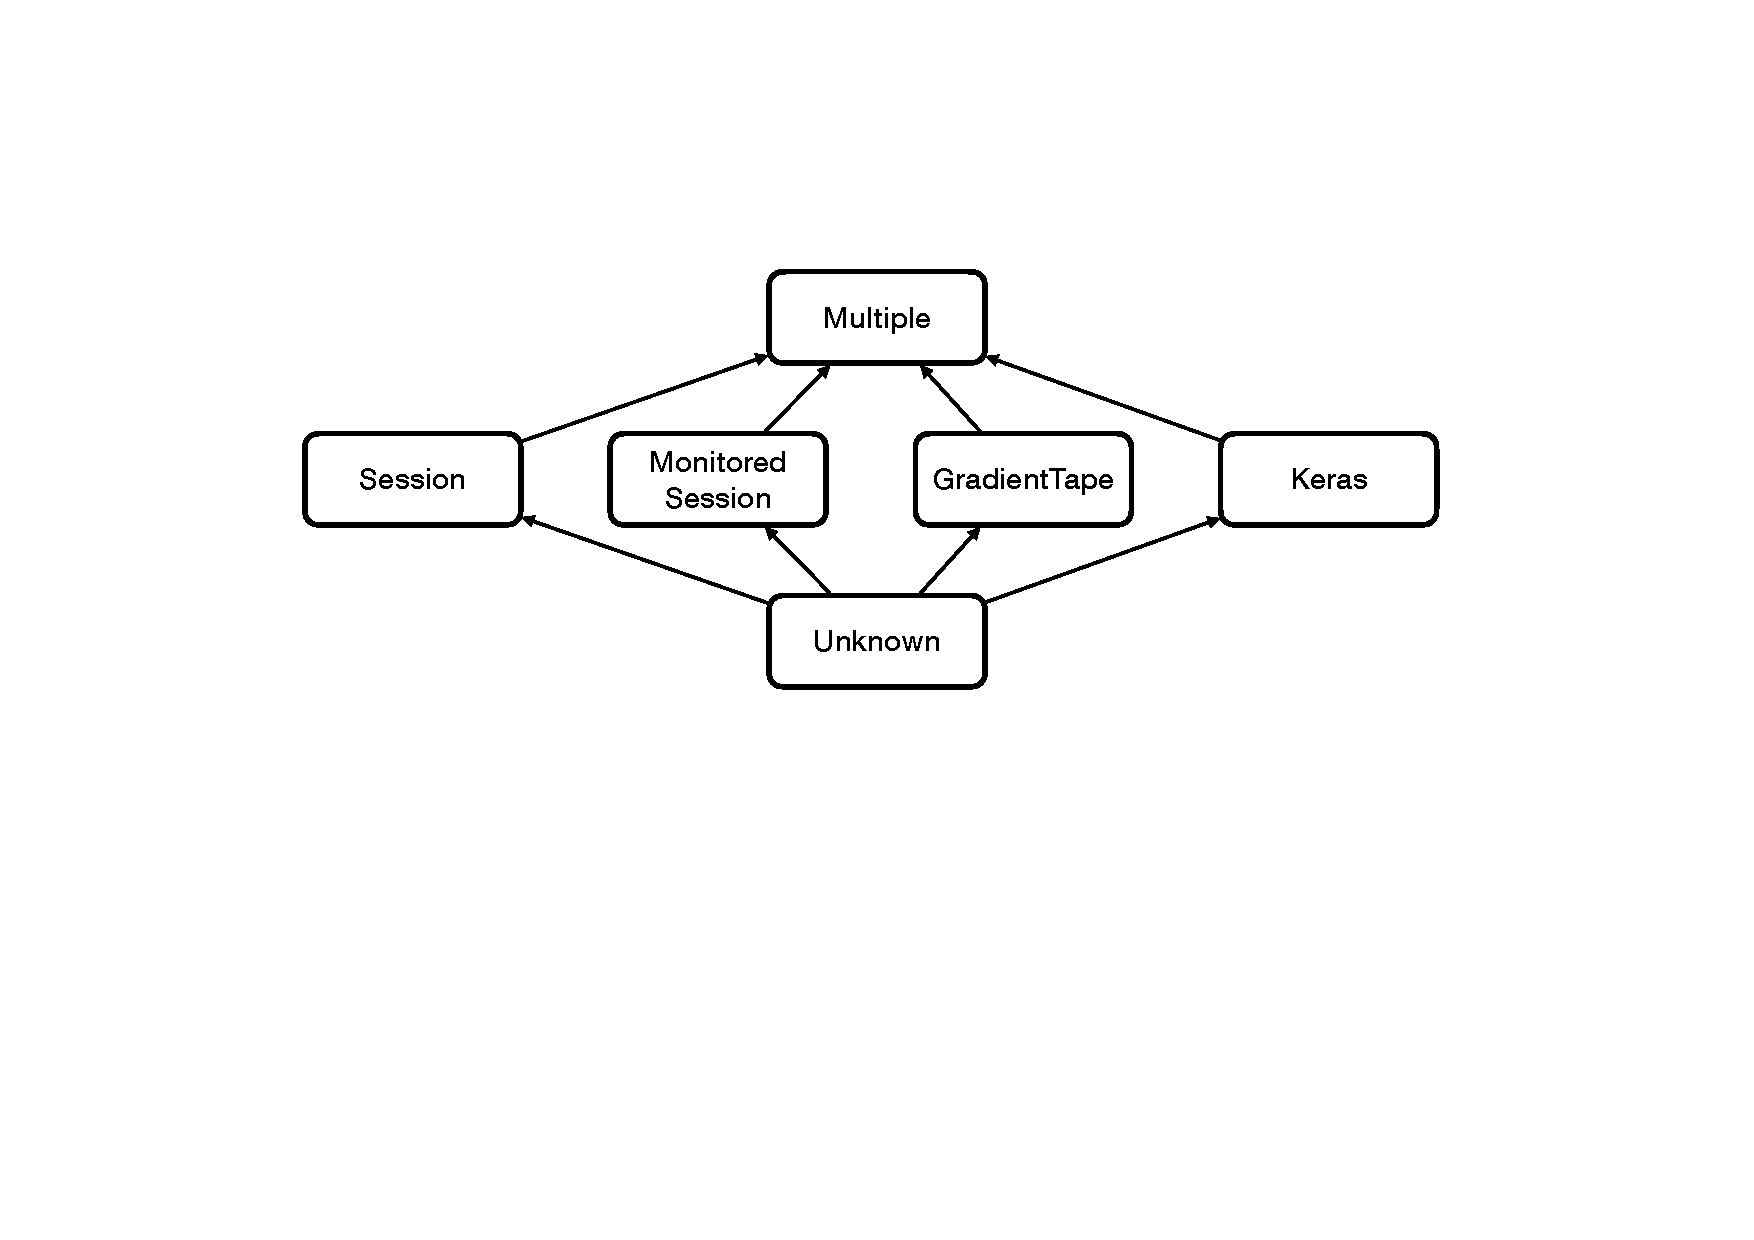
\includegraphics[width=0.7\textwidth]{lattice.pdf}
  \caption{The flat lattice structure of four traininig API patterns}
  \label{fig:pattern:lattice}
\end{figure}


% TODO put algorithm blocks inside the figure env.
% algo related macro
\algblockdefx{Match}{EndMatch}{\textbf{Match}}{}
\algblockdefx{Case}{EndCase}{\textbf{case}}{}
\algtext*{EndMatch}
\algtext*{EndCase}

\algblockdefx{Enum}{EndEnum}{\textbf{Enum}}{}
\algtext*{EndEnum}

% lattice
% \begin{algorithm}[ht!]
%   \caption{Training API pattern lattice}
%   \begin{algorithmic}[1]
%     \Enum~Pattern
%     \State Top
%     \State SessionPattern 
%     \State MonitoredSessionPattern
%     \State GradientTapePattern
%     \State KerasPattern
%     \State Bot
%     \EndEnum
%     
%     \Function{Union}{$x$, $y$} \Comment{Union of two Patterns, x $\cup$ y}
%     \Match~($x$, $y$)~\textbf{with:}
%       \Case~(Bot, $p$) | ($p$, Bot): $p$ \EndCase
%       \Case~\_: Top \EndCase
% 
%     \EndMatch 
%     \EndFunction
%   \end{algorithmic}
%   \label{fig:pattern:algo1}
% \end{algorithm}

% pseudocode
\begin{algorithm}
\caption{Training API pattern identifier}\label{tapa}
  \begin{algorithmic}[1]
    \Function{IdentifyPattern}{$AST$}
    \Match~$AST$~\textbf{with:}

      \Case~{\tt with Session() as}~$name$~{\tt :}~$body$
        \If{$body$~includes~$name${\tt.run()}}
          SessionPattern
        \EndIf
      \EndCase

      \Case~{\tt with MonitoredTrainingSession() as}~$name$~{\tt :}~$body$
        \If{$body$~includes~$name${\tt.run()}}
          MonitoredSessionPattern
        \EndIf
      \EndCase

      \Case~{\tt with GradientTape() as}~$name$~{\tt :}~$body$
        \If{$AST$.parent~includes~$name${\tt.apply\_gradients()}}
          GradientTapePattern
        \EndIf
      \EndCase

      \Case~$model${\tt.fit(...)}
        \If{$model$.class~isSubclassOf~{\tt keras.Model}}
          KerasPattern
        \EndIf
      \EndCase

      \Case~\_
        \If{$AST$.isSimpleStatement}
          Bot 
        \Else
          \State \textbf{Let} childrenPatterns \textbf{=} $AST$.childrenStatements.map(s => IdentifyPattern(s))
          \State childrenPatterns.fold((p1, p2) => p1 $\cup$ p2) 
        \EndIf
      \EndCase

    \EndMatch
    \EndFunction
  \end{algorithmic}
\end{algorithm}

Figure \ref{???} is the pseudocode of the training API pattern identifier.
The function {\tt IdentifyPattern} gets and input AST and returns a training
API pattern lattice element.
The algorithm first matches the statement with four training API patterns.
Lines 3 and 4 match if the input AST is a {\tt with} statement that
creates a {\tt Session} instance and call the {\tt run} method in the body.
If the match succeeds, the algorithm returns Session pattern.
Lines 5 and 6 match if the input AST is a {\tt with} statement that
creates a {\tt MonitoredSession} instance and call the {\tt run} method in the
body.
If the match succeeds, the algorithm returns MonitoredSession pattern.
Line 7 matches if the input AST is a {\tt with} statement that
creates a {\tt GradientTape} instance.
Line 8 then matches if the parent AST has a child statement that calls the
{\tt apply\_gradients} method of the {\tt GradientTape} instance.
If both matches succeed, the algorithm returns GradientTape pattern.
Line 9 and 10 matches if the input AST is a statement that calls
the {\tt fit} method of a subclass of {\tt keras.Model}. 
If the match succeeds, the algorithm returns Keras pattern.

Lines 11 to 15 describe the cases where the input AST does not match with 
one of the four training API patterns.
If the input AST is a simple statement, which does not have child ASTs,
the algorithm returns the bottom element.
Else, the algorithm recursively identifies the pattern of the child ASTs
then return the join of the results.
If the child ASTs are matched with multiple training API patterns, 
the algorithm will return the top element.

\pagebreak
